%%%%%%%%%%%%%%%%%%%%%%%%%%%%%%%%%%%%%%%%%%%%%%
%                insertmeeting
% 1) Title (something creative & funny?)
% 2) Date (MM/DD/YYYY)
% 3) Location (ex. Hagerty High School)
% 4) People/Committees Present 
% 5) Picture 
% 6) Start Time & Stop Time (ex. 12:30AM to 4:30PM)
%%%%%%%%%%%%%%%%%%%%%%%%%%%%%%%%%%%%%%%%%%%%%%
\insertmeeting 
	{Quick Touch Ups} 
	{02/03/22} 
	{Hagerty High School}
	{James, Jensen, Nathan, Ritam}
	{Images/RobotPics/robot.jpg}
	{2:30 - 4:30}
	
\hhscommittee{Hardware}
\noindent\hfil\rule{\textwidth}{.4pt}\hfil
\subsubsection*{Goals}
\begin{itemize}
    \item Review print for driver station and make more adjustments

\end{itemize} 

\noindent\hfil\rule{\textwidth}{.4pt}\hfil

\subsubsection*{Accomplishments}
After the meeting yesterday, we thought we had the station completed but new information was brought up which changed everything. This being that the Acrylic comes in a 12 inch by 12 inch size. This meant that we needed to alter our entire design for the Driver station holder. Our initial thought was to compress everything and make it closer together but that would cause issues with wires and wire management. Instead, we ended up creating a new base which is 11 by 11.5. Our reasoning for this was that our laser cutter has a broken camera and can only cut at a max height of 11.5 though the bed size is a little over 12. This also gave us more room for adjustment and meant we did not have to be as precise. In the end, we decided that instead of having the controllers on opposite sides of the station that it would be better for size if they were on top of each other. This allowed us to be very compact while leaving room for a portable charger so we do not have to worry about our REV Driver Hub from dying during a match. One large change from the initial design to the current design is the use of Velcro instead of Zip Ties. This meant that we would not have to worry about waste and switching parts would be easier to complete. Towards the end of the meeting, we cut the station to determine if there were any errors or changes that needed to be made. We determined that the holes for the Velcro was about 0.1 inches to small and the Driver Hub could be lowered to add more room for cable management.

\begin{figure}[htp]
\centering
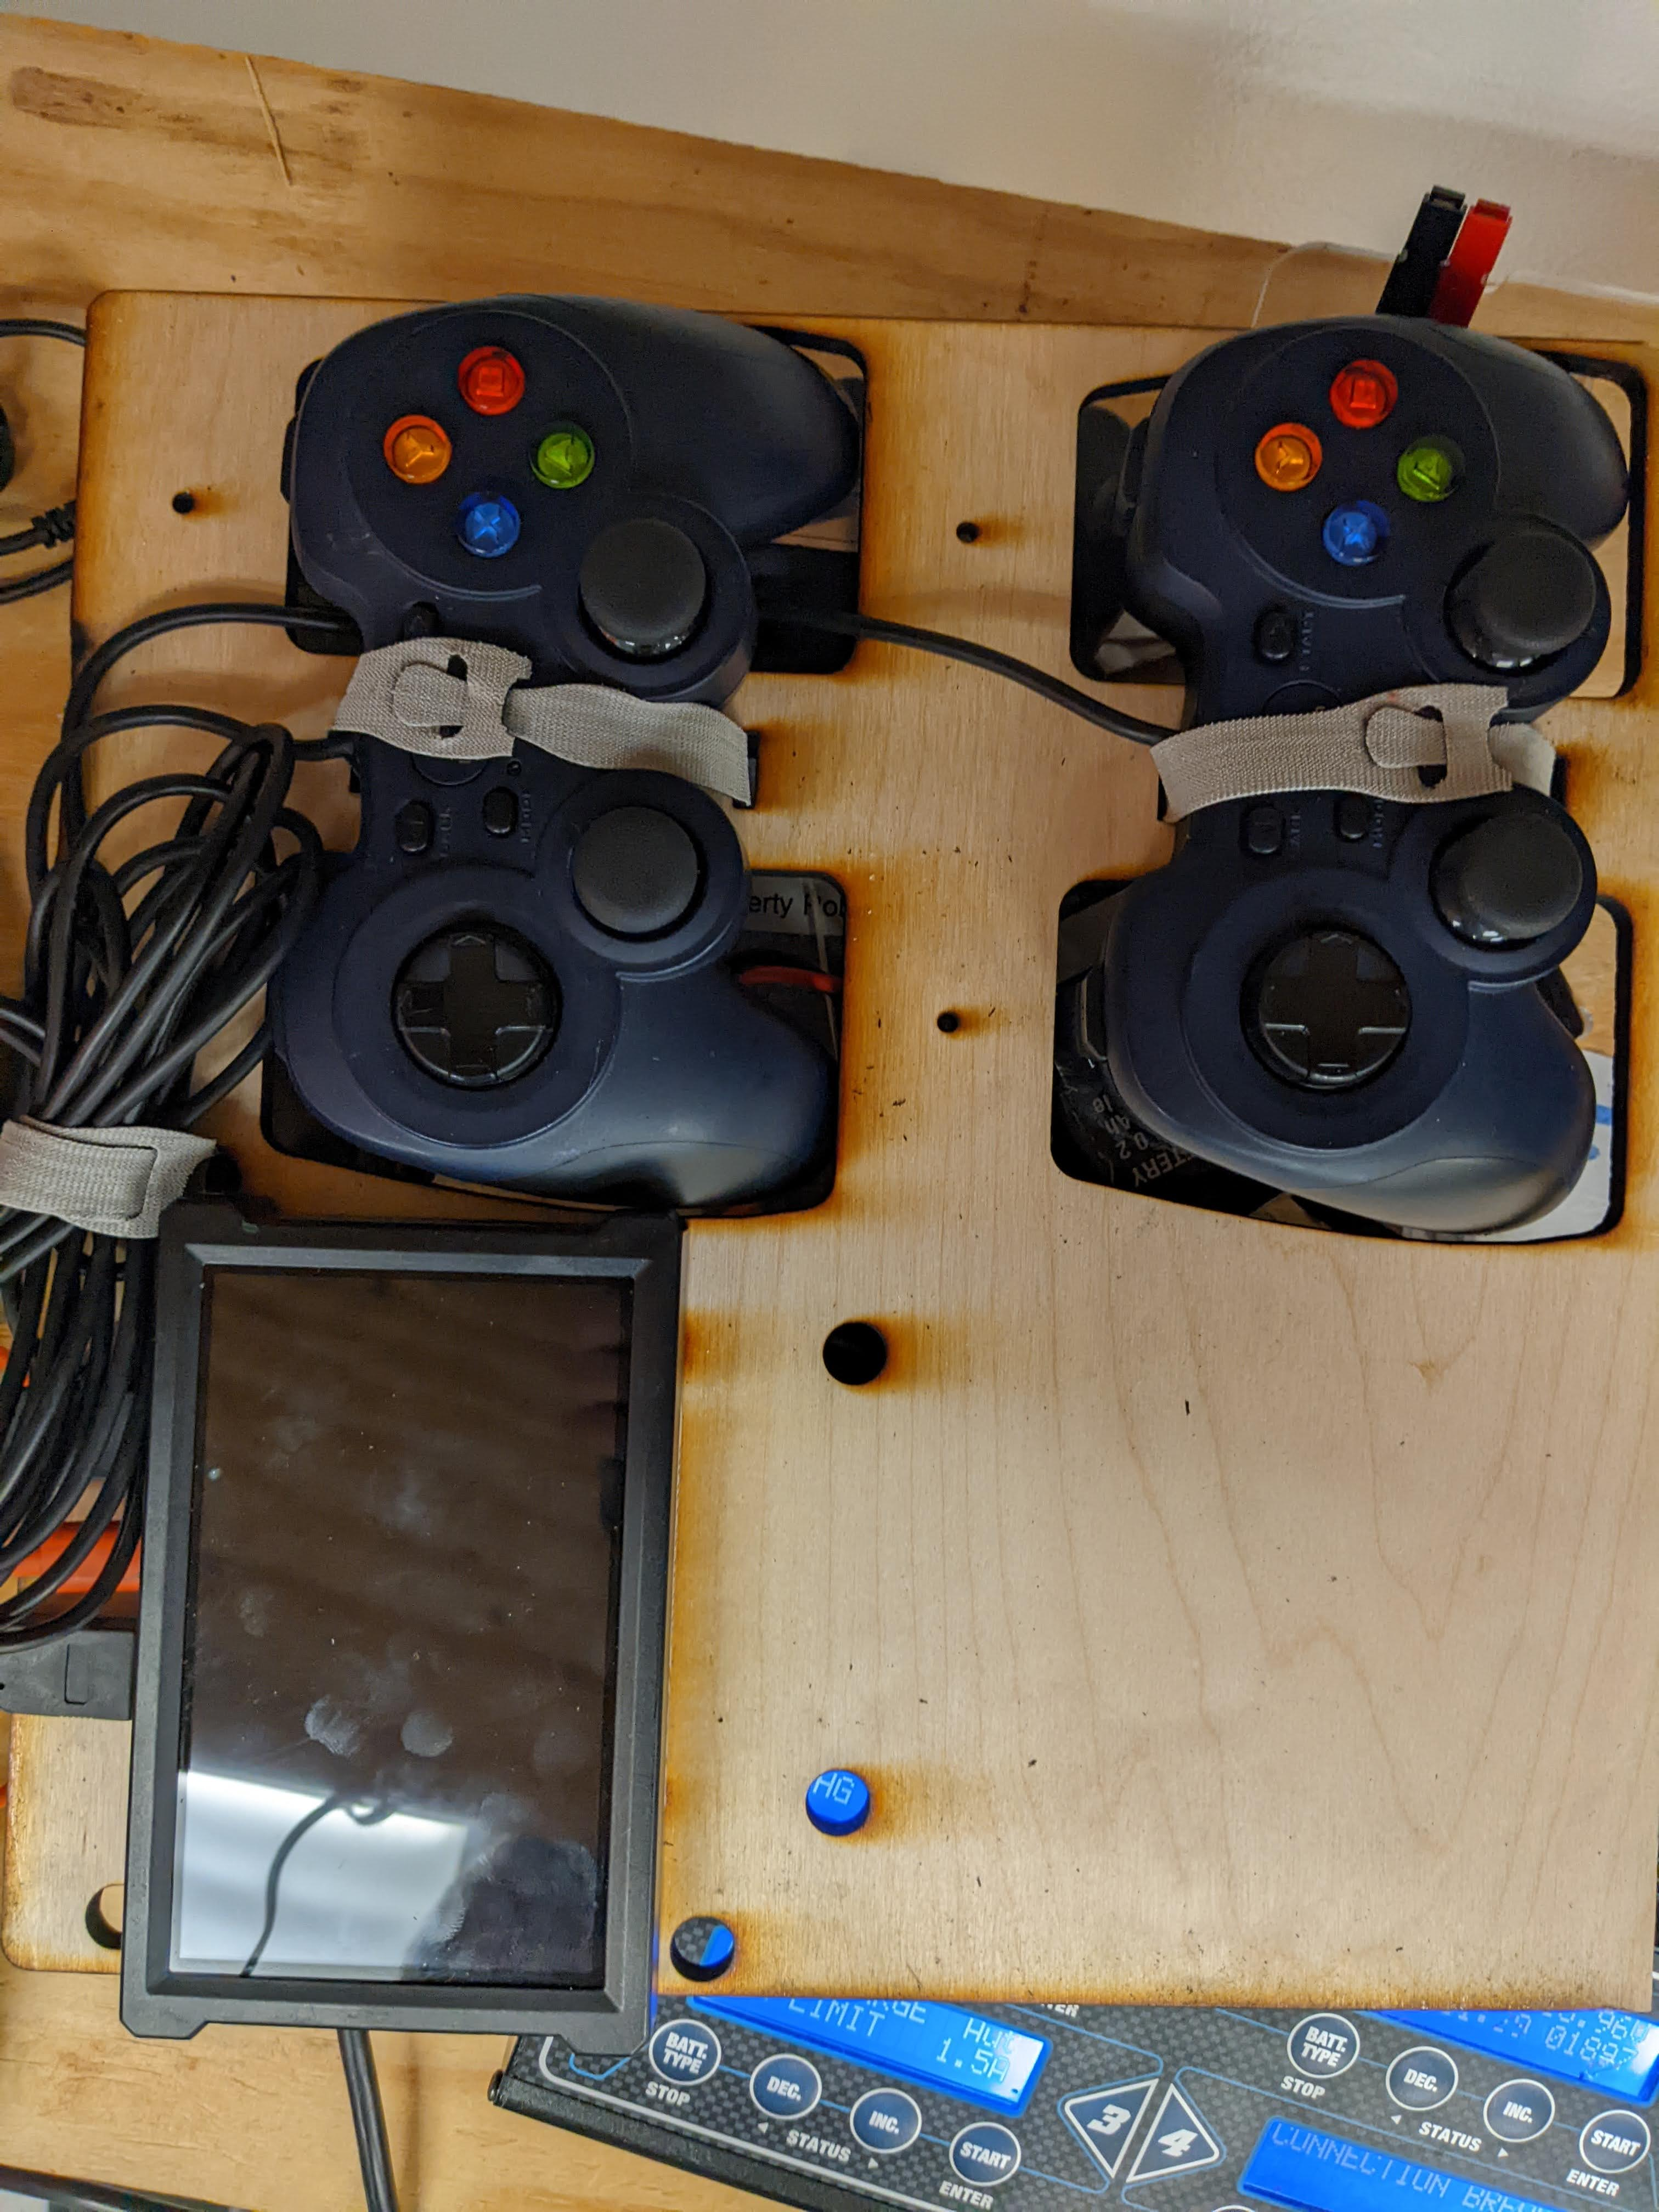
\includegraphics[width=0.95\textwidth, angle=0]{Meetings/February/02-03-22/PXL_20220204_011127244.MP - Jensen Miller.jpg}
\caption{The finished driver station}
\label{fig:pic1}
\end{figure}


\whatsnext{
\begin{itemize}
    \item Get the acrylic to the school and cut the new station
\end{itemize} 
}

